\hypertarget{Introduction}{
}

For human perception, recognizing materials is a very important aspect in our visual system. We can do this flawlessly for a great number of different materials. As a human, we can easily determine whether a surface is smooth, rough, soft or hard by just looking at it. We are also capable of recognizing  materials under great variety of visual conditions. For example, when observing a car from an arbitrary point of view, we always perceive the surface of the car differently when considering the light reflected on the metallic surface which differs from viewpoint to viewpoint. Yet, we have no problem in classifying this surface as metal. The same accounts for many other materials we perceive on a daily base.

Material recognition is a field of research in computer vision with the goal to develop classification systems that can identify various material categories observed in daily life. Examples of such categories are metal, wood, fabric, plastic and glass. Material recognition differs and should not be confused with object recognition and texture recognition. This difference is illustrated in figure \ref{fig:ObjectRecognition} and \ref{fig:TextureRecognition}. A system capable of recognizing materials can greatly enhance the performance of object recognition or scene recognition.

Research has been done on several different material databases and good recognition accuracies have been reported. However, there are suggestions that the accuracies reported are all database dependent \cite{ExploringFeatures} since none of these databases could possibly capture the large variation in appearance of material classes. The large variation of a material class is also addressed as the intra-class variation. 

In this research, we investigate how realistic image synthesis can be employed to create synthetic image data for various material classes. With the aid of image synthesis it is possible to generate infinite amounts of data with arbitrary viewpoint and illumination conditions. This makes it possible to create image data that is not present in material databases, thus making it possible to increase the intra-class variation of material classes.

This chapter gives a short introduction to the problem of material recognition and how image synthesis can be applied to improve recognition performance.

\begin{figure}[htbp!]
	\begin{center}
		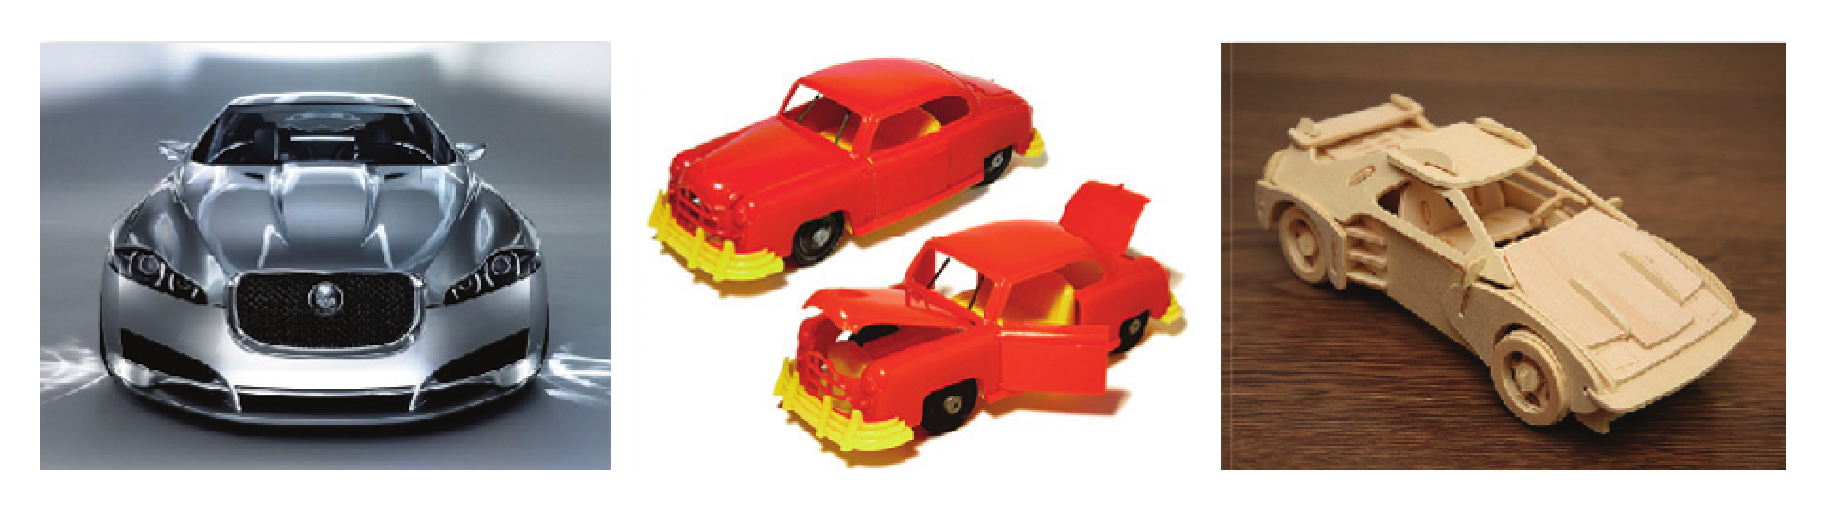
\epsfig{file=images/ObjectRecognition.eps, width=0.6\linewidth}
	\end{center}
	\caption{{\it Object recognition and material recognition: all three pictures depict the same object. However, they are made from metal, plastic and wood respectively. Image adapted from \cite{ExploringFeatures}.}}
	\label{fig:ObjectRecognition}
\end{figure}

\begin{figure}[htbp!]
	\begin{center}
		
\epsfig{file=images/TextureRecognition.eps, width=0.6\linewidth}
	\end{center}
	\caption{{\it Texture recognition and material recognition: all three pictures depict the same pattern. However, they are made from fabric, plastic and paper respectively. Image adapted from \cite{ExploringFeatures}.}}
	\label{fig:TextureRecognition}
\end{figure}

\section{Material Recognition}
Material recognition is defined as the task of correctly classifying a novel image from a material surface. When building a system for material recognition, prediction of a material class is done, preferably, on a single image corresponding to a material surface. This creates a difficult task as the variation in the appearances of materials is considerably enhanced by illumination differences or arbitrary viewpoints. Some examples of how much a surface can vary are shown in figure \ref{fig:PhoTexExamples}.

In recent research, material databases have been created containing various illumination and viewpoint conditions that try to capture the large variety within each  material class. The difficulty is to obtain robust features from the image data that covers various occurrences of materials with different spatial properties as well as distinct illumination properties. 

\begin{figure}[htbp!]
	\begin{center}
		\subfigure[aab]{
\epsfig{file=images/examples/0.aab.0.30.0.eps, width=0.15\linewidth}}\label{fig:aab1}
		\subfigure[acd]{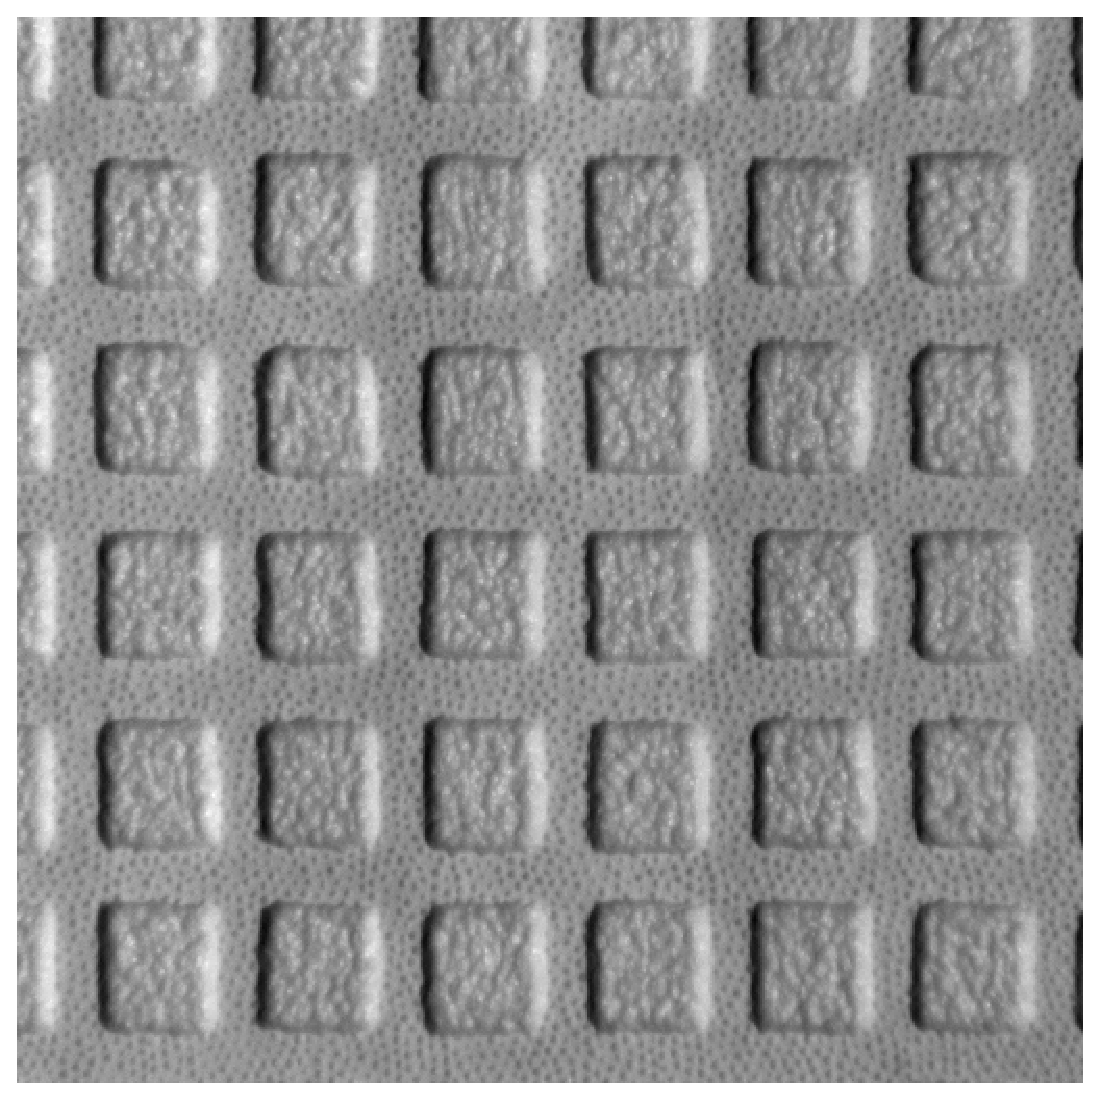
\epsfig{file=images/examples/1.acd.0.30.0.eps, width=0.15\linewidth}}\label{fig:acd1}
		\subfigure[adh]{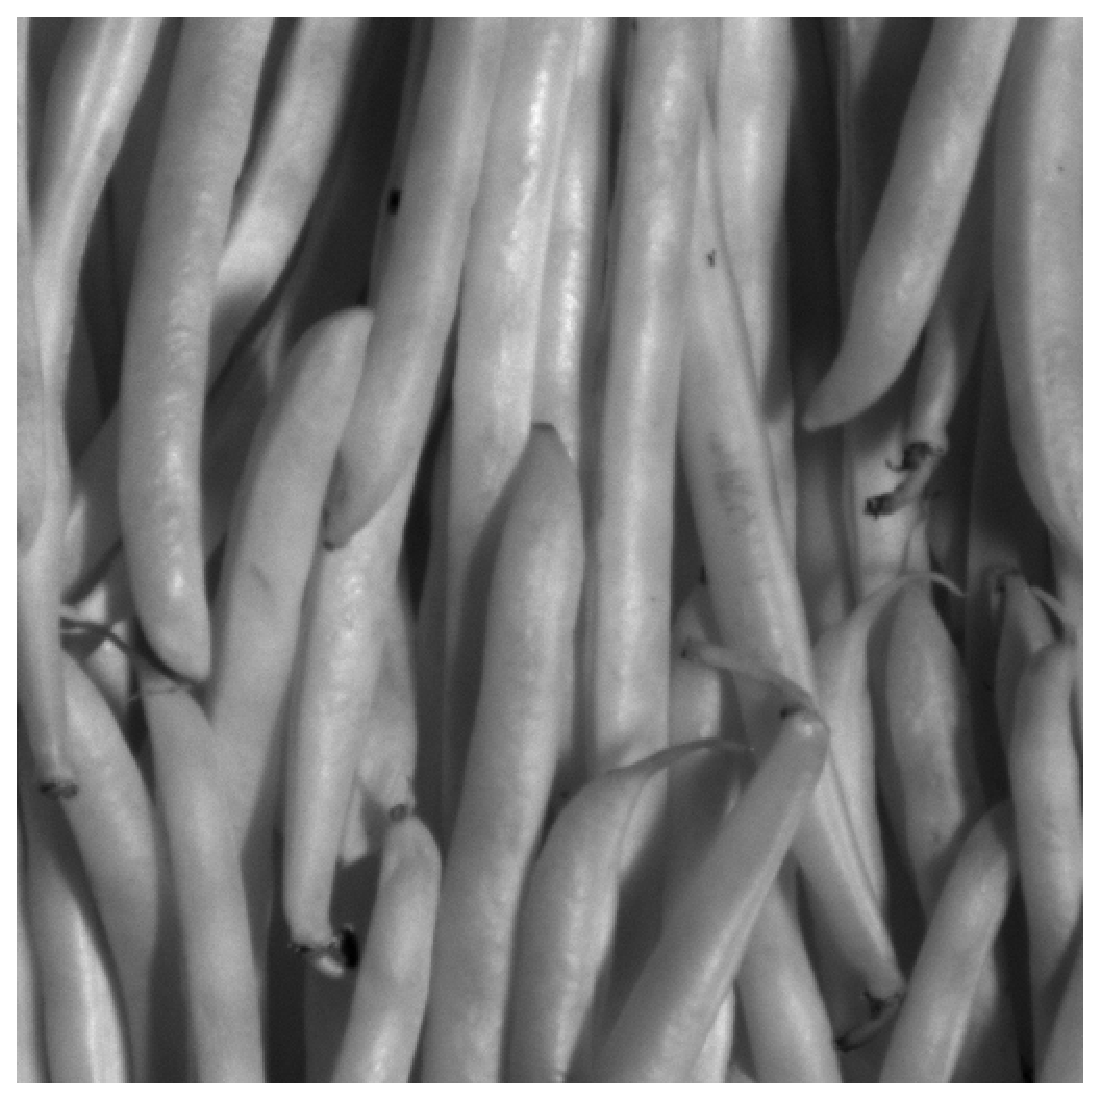
\epsfig{file=images/examples/2.adh.0.30.0.eps, width=0.15\linewidth}}\label{fig:adh1}

		\subfigure[aab]{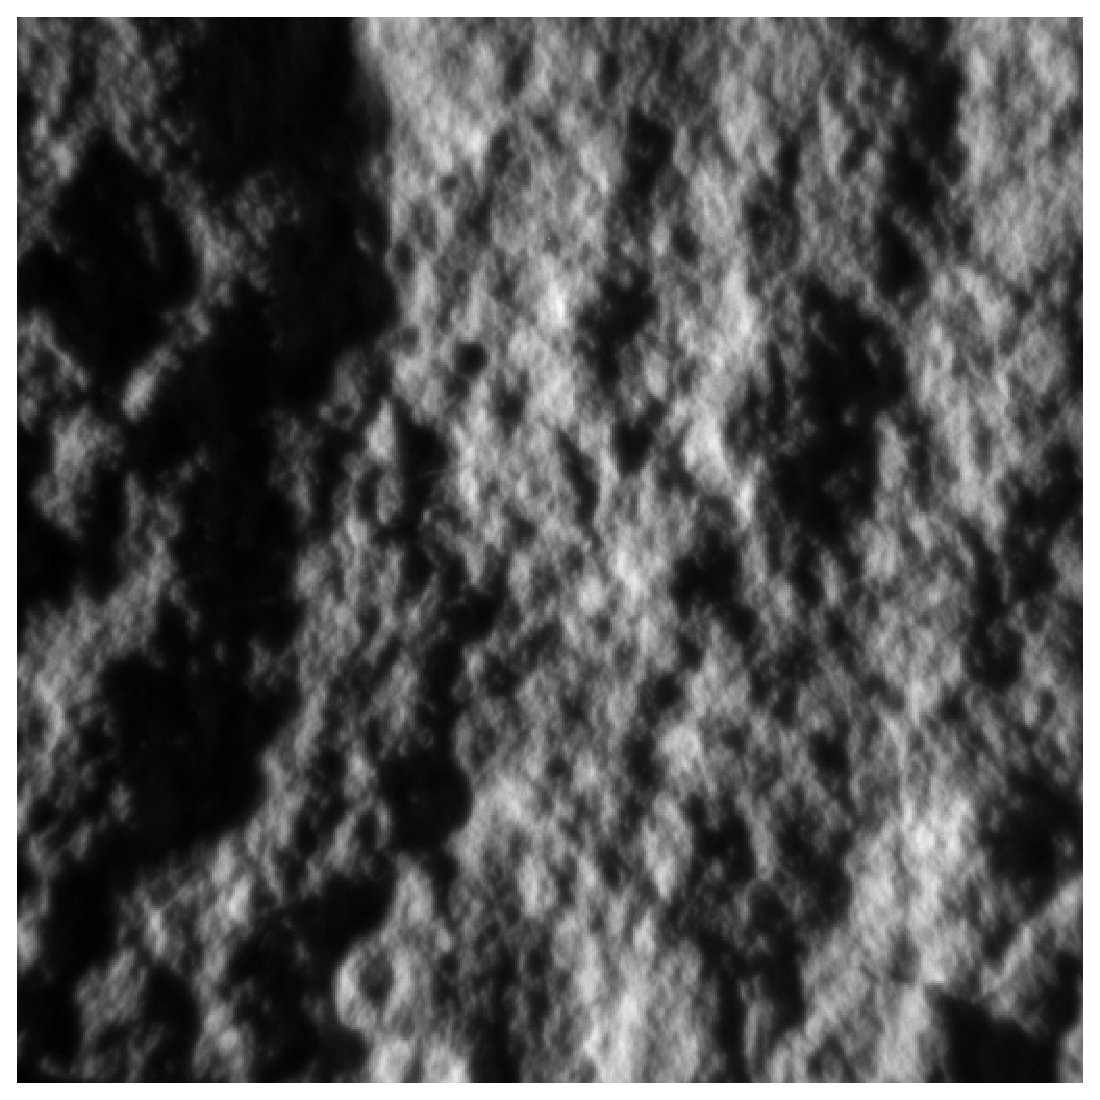
\epsfig{file=images/examples/0.aab.0.75.180.eps, width=0.15\linewidth}}\label{fig:aab2}
		\subfigure[acd]{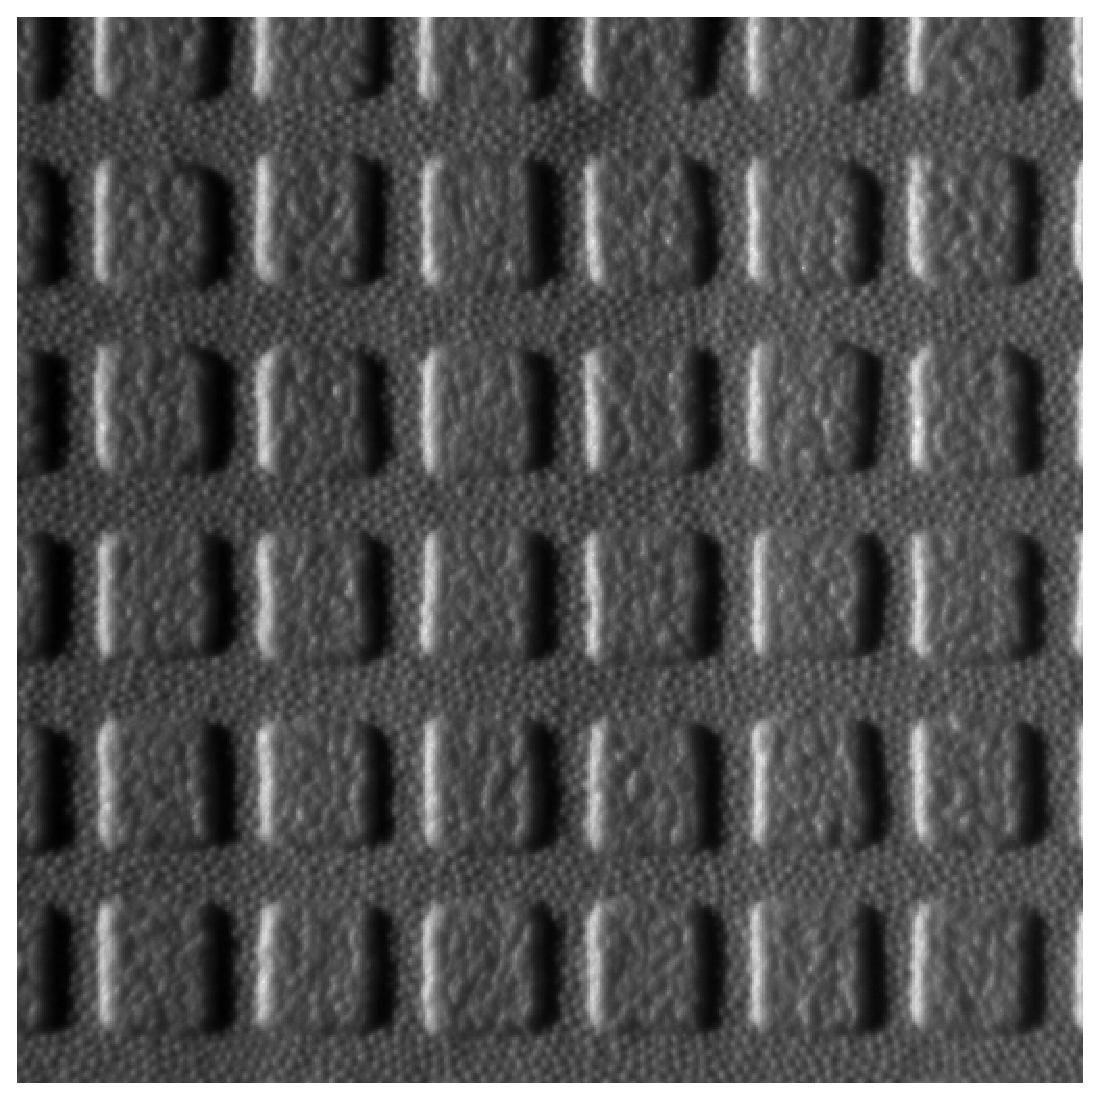
\epsfig{file=images/examples/1.acd.0.75.180.eps, width=0.15\linewidth}}\label{fig:acd2}
		\subfigure[adh]{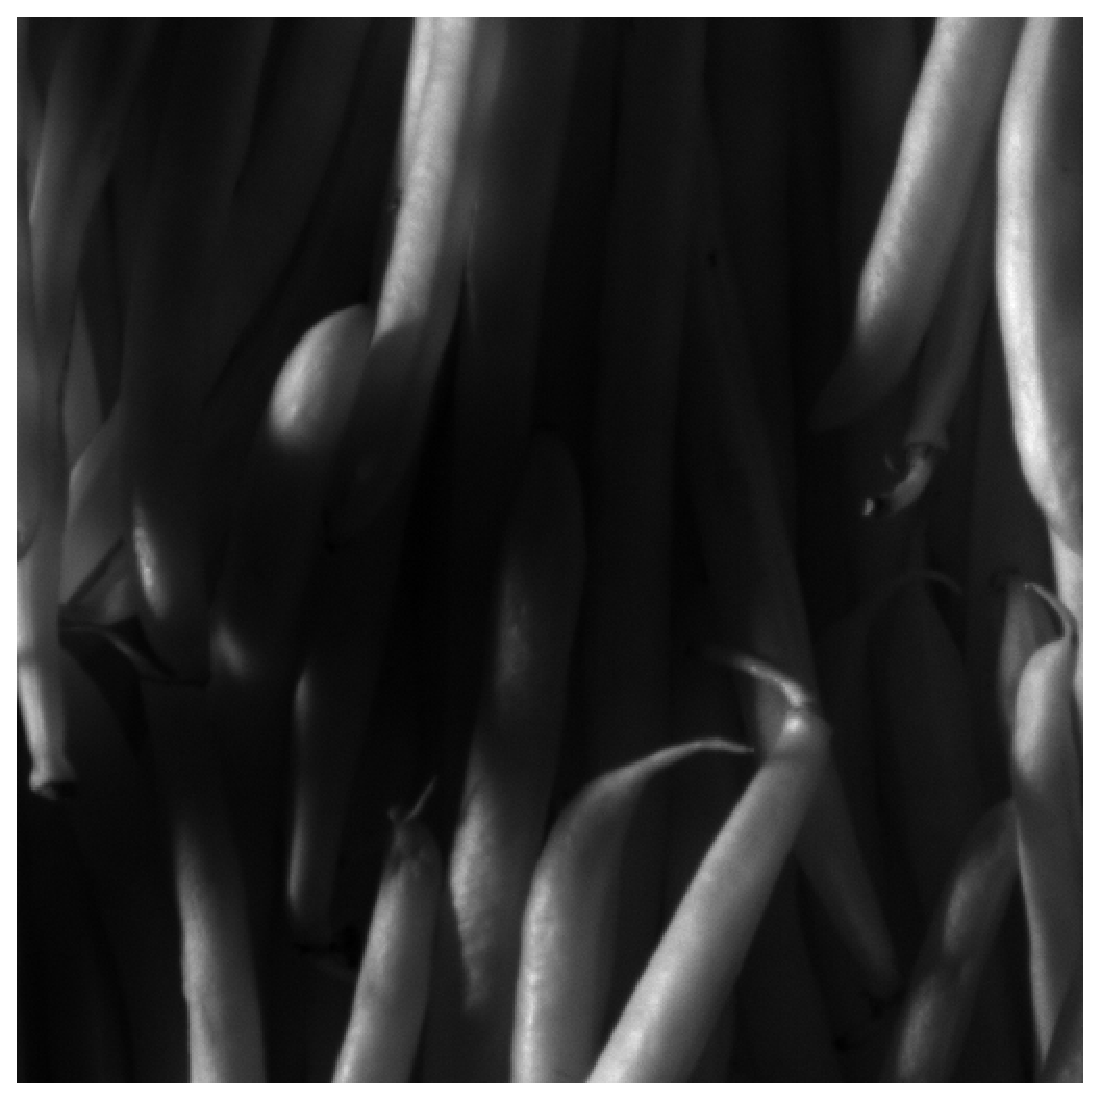
\epsfig{file=images/examples/2.adh.0.75.180.eps, width=0.15\linewidth}}\label{fig:adh2}
	\end{center}
	\caption{{\it Example images from the PhoTex database. The upper row is recorded under a slant of $30^0$ and a tilt of $0^o$. The lower row is recorded under a slant of $75^0$ and a tilt of $180^0$. The captions are the material labels.}}
	\label{fig:PhoTexExamples}
\end{figure}

The {\it CuRET} database captures such properties for 60 different material classes with each over 200 different illumination and viewing directions. This database has been used in the development of texton descriptors to capture the various material properties. In later research on the {\it CuRET} database, parametric models have been developed to deal with the limits of a texton dictionary. The {\it ALOT} and {\it PhoTex} databases have been used in more physically-based computer vision experiments where the geometrical structure of the surface is used for development of robust descriptors. In all these experiments, classification rates of 95\% and higher are reported using various methods such as Naive Bayes, Nearest Neighbor and Support Vector Machines.

The reported classification rates are of great accuracies in general, it seems that most of the difficulties have been solved for material recognition. However, the suggestion that the databases do not capture the intra-class variety for the material classes poses the problem of data shortage. Recording the data is a time-consuming task and will not be sufficiently diverse to capture all possible illumination and viewing directions. 

\section{Image Synthesis}
The field of computer graphics has accomplished imagery of great realism over the past few decades. With increasing computational power, it became possible to synthesize realistic images using expensive physically-based light simulations. 

Various models have been developed for the synthesis of diffuse, glossy or shiny materials. These models use as input for per-pixel generation of an image a surface normal, the surface albedo, a viewing direction, an illumination direction and illumination properties such as the color of the light source. With proper reconstruction of the surface normals and surface albedo for a material, it is possible to generate an infinite amount of data with arbitrary viewing and illumination directions. Databases such as {\it PhoTex} and {\it ALOT} were created with physically-based computer vision in mind. With image data available for each material class with recorded light source directions, it is possible to recover surface normals and surface albedo for material classes. 

In research done by Targhi \cite{Targhi}, the synthesis of material images has been used to augment training-sets to a point of saturation where perfect predictions were made \cite{Targhi}. For the synthesis of image data, the Lambertian reflection model was used. This reflection model is limited to the synthesis of purely diffuse materials only, since the reflection model does not simulate illumination phenomena such as speculars which are observed on glossy and shiny surfaces. Other reflection models should be considered as well if we want to be able to synthesize images for other than purely diffuse materials.

\section{Goal of this thesis}
In this research, the aim is to investigate the addition of more sophisticated reflection models for the synthesis of realistic image data. We research and implement combinations of Lambertian reflectance with models for speculars such as Phong, Blinn-Phong and Torrance-Sparrow, as well as a more sophisticated model for diffuse reflection. 

The synthetic image data is used for training models for material classification. These models are tested against two datasets: a dataset consisting of mainly diffuse materials and a dataset consisting of shiny/glossy materials. Our main focus is to test and compare performance of classification when using only synthetic image data for training the models for classification. With the addition of specular reflection models for synthesis, we can expect some improved models when comparing the performance with models obtained from synthetic data using Lambertian reflection only.

\section{Overview of this thesis}
In the next chapter, some of the state-of-the-art methods and their experiments are outlined. Some of these methods are adapted for the experiments in this research. Chapter 3 outlines some fundamentals that are used for understanding local reflection models. In chapter 4 the methods and data that we adapt in this research will be discussed in more detail. In chapter 5, a set of empirical reflection models that we have implemented for the experiments are presented in detail. In chapter 6, a set of more physical-based reflection models that we implemented are discussed in detail. In chapter 7, the experiments and their results are reported and the last chapter holds the conclusion and future works.

